\documentclass[8pt]{beamer}

% Beamer style
%\usetheme[secheader]{Madrid}
% \usetheme{CambridgeUS}
\useoutertheme{infolines}
\usecolortheme[rgb={0.65,0.15,0.25}]{structure}
% \usefonttheme[onlymath]{serif}
\beamertemplatenavigationsymbolsempty
%\AtBeginSubsection

% Packages
%\usepackage[french]{babel}
\usepackage[latin1]{inputenc}
\usepackage{color}
% \usepackage[dvipsnames]{xcolor}
\usepackage{xspace}
\usepackage{dsfont, stmaryrd}
\usepackage{amsmath, amsfonts, amssymb, stmaryrd, mathabx}
\usepackage{epsfig}
\usepackage{tikz}
\usepackage{url}
% \usepackage{ulem}
\usepackage{/home/robin/LATEX/Biblio/astats}
%\usepackage[all]{xy}
\usepackage{graphicx}

% Maths
% \newtheorem{theorem}{Theorem}
% \newtheorem{definition}{Definition}
\newtheorem{proposition}{Proposition}
% \newtheorem{assumption}{Assumption}
% \newtheorem{algorithm}{Algorithm}
% \newtheorem{lemma}{Lemma}
% \newtheorem{remark}{Remark}
% \newtheorem{exercise}{Exercise}
% \newcommand{\propname}{Prop.}
% \newcommand{\proof}{\noindent{\sl Proof:}\quad}
% \newcommand{\eproof}{$\blacksquare$}

% \setcounter{secnumdepth}{3}
% \setcounter{tocdepth}{3}
\newcommand{\pref}[1]{\ref{#1} p.\pageref{#1}}
\newcommand{\qref}[1]{\eqref{#1} p.\pageref{#1}}

% Colors : http://latexcolor.com/
\definecolor{darkred}{rgb}{0.65,0.15,0.25}
\definecolor{darkgreen}{rgb}{0,0.4,0}
\definecolor{darkred}{rgb}{0.65,0.15,0.25}
\definecolor{amethyst}{rgb}{0.6, 0.4, 0.8}
\definecolor{asparagus}{rgb}{0.53, 0.66, 0.42}
\definecolor{applegreen}{rgb}{0.55, 0.71, 0.0}
\definecolor{awesome}{rgb}{1.0, 0.13, 0.32}
\definecolor{blue-green}{rgb}{0.0, 0.87, 0.87}
\definecolor{red-ggplot}{rgb}{0.52, 0.25, 0.23}
\definecolor{green-ggplot}{rgb}{0.42, 0.58, 0.00}
\definecolor{purple-ggplot}{rgb}{0.34, 0.21, 0.44}
\definecolor{blue-ggplot}{rgb}{0.00, 0.49, 0.51}

% Commands
\newcommand{\backupbegin}{
   \newcounter{finalframe}
   \setcounter{finalframe}{\value{framenumber}}
}
\newcommand{\backupend}{
   \setcounter{framenumber}{\value{finalframe}}
}
\newcommand{\emphase}[1]{\textcolor{darkred}{#1}}
\newcommand{\comment}[1]{\textcolor{gray}{#1}}
\newcommand{\paragraph}[1]{\textcolor{darkred}{#1}}
\newcommand{\refer}[1]{{\small{\textcolor{gray}{{\cite{#1}}}}}}
\newcommand{\Refer}[1]{{\small{\textcolor{gray}{{[#1]}}}}}
\newcommand{\goto}[1]{{\small{\textcolor{blue}{[\#\ref{#1}]}}}}
\renewcommand{\newblock}{}

\newcommand{\tabequation}[1]{{\medskip \centerline{#1} \medskip}}
% \renewcommand{\binom}[2]{{\left(\begin{array}{c} #1 \\ #2 \end{array}\right)}}

% Variables 
\newcommand{\Abf}{{\bf A}}
\newcommand{\Beta}{\text{B}}
\newcommand{\Bcal}{\mathcal{B}}
\newcommand{\Bias}{\xspace\mathbb B}
\newcommand{\Cor}{{\mathbb C}\text{or}}
\newcommand{\Cov}{{\mathbb C}\text{ov}}
\newcommand{\cl}{\text{\it c}\ell}
\newcommand{\Ccal}{\mathcal{C}}
\newcommand{\cst}{\text{cst}}
\newcommand{\Dcal}{\mathcal{D}}
\newcommand{\Ecal}{\mathcal{E}}
\newcommand{\Esp}{\xspace\mathbb E}
\newcommand{\Espt}{\widetilde{\Esp}}
\newcommand{\Covt}{\widetilde{\Cov}}
\newcommand{\Ibb}{\mathbb I}
\newcommand{\Fcal}{\mathcal{F}}
\newcommand{\Gcal}{\mathcal{G}}
\newcommand{\Gam}{\mathcal{G}\text{am}}
\newcommand{\Hcal}{\mathcal{H}}
\newcommand{\Jcal}{\mathcal{J}}
\newcommand{\Lcal}{\mathcal{L}}
\newcommand{\Mt}{\widetilde{M}}
\newcommand{\mt}{\widetilde{m}}
\newcommand{\Nbb}{\mathbb{N}}
\newcommand{\Mcal}{\mathcal{M}}
\newcommand{\Ncal}{\mathcal{N}}
\newcommand{\Ocal}{\mathcal{O}}
\newcommand{\pt}{\widetilde{p}}
\newcommand{\Pt}{\widetilde{P}}
\newcommand{\Pbb}{\mathbb{P}}
\newcommand{\Pcal}{\mathcal{P}}
\newcommand{\Qcal}{\mathcal{Q}}
\newcommand{\qt}{\widetilde{q}}
\newcommand{\Rbb}{\mathbb{R}}
\newcommand{\Sbb}{\mathbb{S}}
\newcommand{\Scal}{\mathcal{S}}
\newcommand{\st}{\widetilde{s}}
\newcommand{\St}{\widetilde{S}}
\newcommand{\Tcal}{\mathcal{T}}
\newcommand{\todo}{\textcolor{red}{TO DO}}
\newcommand{\Ucal}{\mathcal{U}}
\newcommand{\Un}{\math{1}}
\newcommand{\Vcal}{\mathcal{V}}
\newcommand{\Var}{\mathbb V}
\newcommand{\Vart}{\widetilde{\Var}}
\newcommand{\Zcal}{\mathcal{Z}}

% Symboles & notations
\newcommand\independent{\protect\mathpalette{\protect\independenT}{\perp}}\def\independenT#1#2{\mathrel{\rlap{$#1#2$}\mkern2mu{#1#2}}} 
\renewcommand{\d}{\text{\xspace d}}
\newcommand{\gv}{\mid}
\newcommand{\ggv}{\, \| \, }
% \newcommand{\diag}{\text{diag}}
\newcommand{\card}[1]{\text{card}\left(#1\right)}
\newcommand{\trace}[1]{\text{tr}\left(#1\right)}
\newcommand{\matr}[1]{\boldsymbol{#1}}
\newcommand{\matrbf}[1]{\mathbf{#1}}
\newcommand{\vect}[1]{\matr{#1}} %% un peu inutile
\newcommand{\vectbf}[1]{\matrbf{#1}} %% un peu inutile
\newcommand{\trans}{\intercal}
\newcommand{\transpose}[1]{\matr{#1}^\trans}
\newcommand{\crossprod}[2]{\transpose{#1} \matr{#2}}
\newcommand{\tcrossprod}[2]{\matr{#1} \transpose{#2}}
\newcommand{\matprod}[2]{\matr{#1} \matr{#2}}
\DeclareMathOperator*{\argmin}{arg\,min}
\DeclareMathOperator*{\argmax}{arg\,max}
\DeclareMathOperator{\sign}{sign}
\DeclareMathOperator{\tr}{tr}
\newcommand{\ra}{\emphase{$\rightarrow$} \xspace}

% Hadamard, Kronecker and vec operators
\DeclareMathOperator{\Diag}{Diag} % matrix diagonal
\DeclareMathOperator{\diag}{diag} % vector diagonal
\DeclareMathOperator{\mtov}{vec} % matrix to vector
\newcommand{\kro}{\otimes} % Kronecker product
\newcommand{\had}{\odot}   % Hadamard product

% TikZ
\newcommand{\nodesize}{2em}
\newcommand{\edgeunit}{2.5*\nodesize}
\newcommand{\edgewidth}{1pt}
\tikzstyle{node}=[draw, circle, fill=black, minimum width=.75\nodesize, inner sep=0]
\tikzstyle{square}=[rectangle, draw]
\tikzstyle{param}=[draw, rectangle, fill=gray!50, minimum width=\nodesize, minimum height=\nodesize, inner sep=0]
\tikzstyle{hidden}=[draw, circle, fill=gray!50, minimum width=\nodesize, inner sep=0]
\tikzstyle{hiddenred}=[draw, circle, color=red, fill=gray!50, minimum width=\nodesize, inner sep=0]
\tikzstyle{observed}=[draw, circle, minimum width=\nodesize, inner sep=0]
\tikzstyle{observedred}=[draw, circle, minimum width=\nodesize, color=red, inner sep=0]
\tikzstyle{eliminated}=[draw, circle, minimum width=\nodesize, color=gray!50, inner sep=0]
\tikzstyle{empty}=[draw, circle, minimum width=\nodesize, color=white, inner sep=0]
\tikzstyle{blank}=[color=white]
\tikzstyle{nocircle}=[minimum width=\nodesize, inner sep=0]

\tikzstyle{edge}=[-, line width=\edgewidth]
\tikzstyle{edgebendleft}=[-, >=latex, line width=\edgewidth, bend left]
\tikzstyle{edgebendright}=[-, >=latex, line width=\edgewidth, bend right]
\tikzstyle{lightedge}=[-, line width=\edgewidth, color=gray!50]
\tikzstyle{lightedgebendleft}=[-, >=latex, line width=\edgewidth, bend left, color=gray!50]
\tikzstyle{lightedgebendright}=[-, >=latex, line width=\edgewidth, bend right, color=gray!50]
\tikzstyle{edgered}=[-, line width=\edgewidth, color=red]
\tikzstyle{edgebendleftred}=[-, >=latex, line width=\edgewidth, bend left, color=red]
\tikzstyle{edgebendrightred}=[-, >=latex, line width=\edgewidth, bend right, color=red]

\tikzstyle{arrow}=[->, >=latex, line width=\edgewidth]
\tikzstyle{arrowbendleft}=[->, >=latex, line width=\edgewidth, bend left]
\tikzstyle{arrowbendright}=[->, >=latex, line width=\edgewidth, bend right]
\tikzstyle{arrowred}=[->, >=latex, line width=\edgewidth, color=red]
\tikzstyle{arrowbendleftred}=[->, >=latex, line width=\edgewidth, bend left, color=red]
\tikzstyle{arrowbendrightred}=[->, >=latex, line width=\edgewidth, bend right, color=red]
\tikzstyle{arrowblue}=[->, >=latex, line width=\edgewidth, color=blue]
\tikzstyle{dashedarrow}=[->, >=latex, dashed, line width=\edgewidth]
\tikzstyle{dashededge}=[-, >=latex, dashed, line width=\edgewidth]
\tikzstyle{dashededgebendleft}=[-, >=latex, dashed, line width=\edgewidth, bend left]
\tikzstyle{lightarrow}=[->, >=latex, line width=\edgewidth, color=gray!50]

\newcommand{\dN}{\Delta N}
\newcommand{\dtau}{\Delta \tau}

% Directory
\newcommand{\figcp}{/home/robin/RECHERCHE/RUPTURES/EXPOSES/FIGURES}

%====================================================================
%====================================================================

%====================================================================
%====================================================================
\begin{document}
%====================================================================
%====================================================================

%====================================================================
\title[Segmentation of point processes]{Segmentation (and classification) of point processes}

\author[S. Robin]{S. Robin \\ \medskip
joint work with C. Dion-Blanc \& E. Lebarbier and A. Bonnet \& C. Matias}

\institute[]{Sorbonne universit�}

\date[HCERES]{HCERES, LPSM, Dec. 2023}

%====================================================================
%====================================================================
\maketitle

% %====================================================================
% %====================================================================
% \section{Change-point detection}
%====================================================================
\frame{\frametitle{Change-point detection} 

  \begin{tabular}{cc}
    \hspace{-.04\textwidth}
    \begin{tabular}{p{.5\textwidth}}
      \onslide+<1->{\paragraph{Point process on $t \in [0, 1]$.} \\
      Event times:
      $$
      0 < T_1 < \dots T_i < \dots T_n < 1;
      $$ 
      Counting process:
      $$
      N(t) = \sum_{i=1}^n \Ibb\{T_i \leq t\}.
      $$}      
      
      \bigskip \pause
      \onslide+<3->{\paragraph{Change-point detection.} \\
      Look for times
      $$
      0 < \tau_1 < \dots < \tau_{K-1} < 1
      $$
      where the distribution of $N$ changes abruptly.}

    \end{tabular}
    & 
    \hspace{-.02\textwidth}
    \begin{tabular}{p{.5\textwidth}}
      \begin{overprint}
          \onslide<2>
          \paragraph{Bat cries} (night of the 17 jul. 2019)\footnote{source: Vigie-Chiro program, CESCO-MNHN} \\
          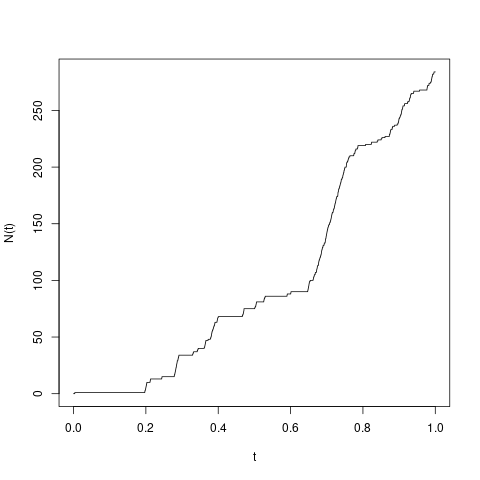
\includegraphics[width=.45\textwidth, trim=0 10 0 50, clip=]{\figcp/FigSegPP-Chiroptere-seq2295-day2019-07-17-Path}
          \onslide<3>
          \paragraph{Bat cries} (night of the 17 jul. 2019)\footnote{source: Vigie-Chiro program, CESCO-MNHN} \\
          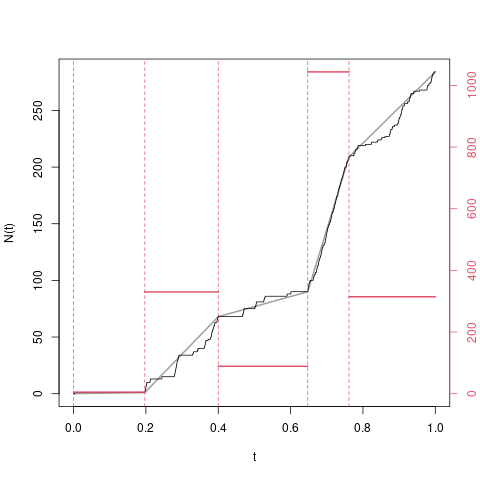
\includegraphics[width=.45\textwidth, trim=0 10 0 50, clip=]{\figcp/FigSegPP-Chiroptere-seq2295-day2019-07-17-Seg}
          \onslide<4>
          \paragraph{Kilauea's eruptions} (from 1750 to 1984)\footnote{source: \refer{HoB17}} \\
          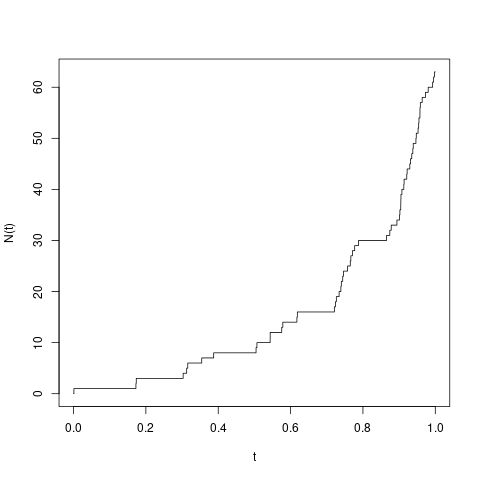
\includegraphics[width=.45\textwidth, trim=0 10 0 50, clip=]{\figcp/FigSegPP-Kilauea-Path}
          \onslide<5>
          \paragraph{Kilauea's eruptions} (from 1750 to 1984)\footnote{source: \refer{HoB17}}  \\
          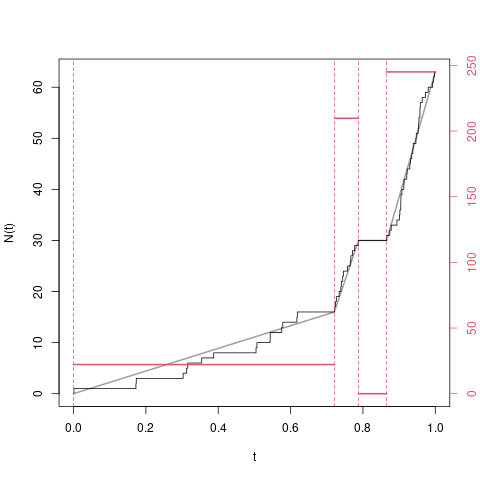
\includegraphics[width=.45\textwidth, trim=0 10 0 50, clip=]{\figcp/FigSegPP-Kilauea-Seg}
      \end{overprint}
    \end{tabular}
  \end{tabular}

}

%====================================================================
\frame{\frametitle{Change-point detection} 

  \paragraph{Three typical steps.}
  \begin{enumerate}
    \setlength{\itemsep}{1\baselineskip}
    \item Propose a set of reasonably realistic models;
    \item Design an (efficient) algorithm to get the parameter estimates;
    \item Choose among the models.
  \end{enumerate}

  \bigskip \bigskip \pause
  \paragraph{Example.}
  \begin{enumerate}
    \setlength{\itemsep}{1.25\baselineskip}
    \item $N(t)$ is a Poisson process with piece-wise constant intensity function $\lambda$:
    $$
    \lambda(t) = \lambda_k \qquad \text{if} \quad \tau_{k-1} \leq t < \tau_k.
    $$
    Parameters: change-points $\tau =  (\tau_k)_{1 \leq k \leq K-1}$ and intensities $\lambda = (\lambda_k)_{1 \leq k \leq K}$.
    \item For a given number of segments $K$ find 
    $$
    (\widehat{\lambda}, \widehat{\tau}) = \arg\min_{\tau, \lambda} C_K(N; \tau, \lambda), 
    \qquad \text{e.g.} \quad 
    C_K(N; \tau, \lambda) = - \log p_{K, \tau, \lambda}(N);
    $$
    \item Choose the number of segments $K$.
  \end{enumerate}

}

%====================================================================
\frame{\frametitle{Change-point detection} 

  \begin{tabular}{cc}
    \hspace{-.04\textwidth}
    \begin{tabular}{p{.56\textwidth}}
      \paragraph{Discrete-time.} 
      \begin{itemize}
        \setlength{\itemsep}{1\baselineskip}
        \item Data = $\{Y_t\}_{t = 1, \dots n}$ (independent); 
        \item Change-points: $\tau \in \Tcal \subset \llbracket n-1 \rrbracket^{K-1}$;
        \item $\tau_{k-1} < t \leq \tau_k$: $Y_t \sim \Ncal(\mu_k, 1)$.
      \end{itemize}
      
      \bigskip
      Parameters:
      $\mu_k$ continuous, $\tau_k$ discrete.
      
    \end{tabular}
    & 
    \hspace{-.1\textwidth}
    \begin{tabular}{p{.45\textwidth}}
      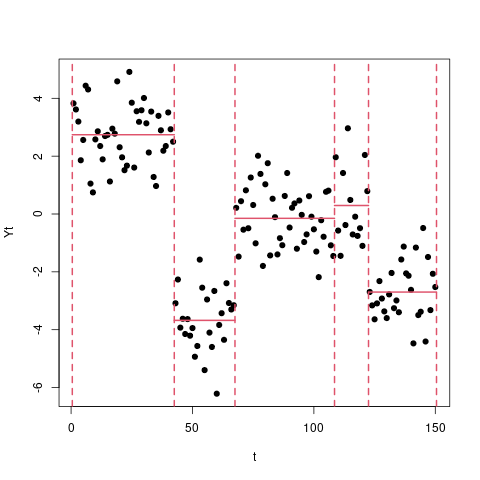
\includegraphics[width=.45\textwidth, trim=0 10 0 10, clip=]{\figcp/FigSeg-HCERES-discrete-seg}
    \end{tabular}
  \end{tabular}
  
  \pause
  $\Tcal =$ 'segmentation space':
  $$
  \Tcal = \{\tau \in \llbracket n-1 \rrbracket^{K-1}: 
  1 \leq \tau_1 < \dots \tau_{K-1} < n\}, 
  \qquad
  \text{card}(\Tcal) = {{n-1}\choose{K-1}}.
  $$
  \emphase{Dynamic programming (DP)} recovers the optimal $\widehat{\tau}_k$ in $O(n^2)$ (or less), as long as the contrast (e.g. neg-log-likelihood) is additive \refer{AuL89}.
  
}

% %====================================================================
% %====================================================================
% \section{Change-point detection in a Poisson process}
%====================================================================
\frame{\frametitle{Change-point detection in a Poisson process} 

  \bigskip
  \paragraph{Model.} Poisson process with piece-wise constant intensity.

  \bigskip
  \begin{tabular}{cc}
    \hspace{-.04\textwidth}
    \begin{tabular}{p{.5\textwidth}}
      \paragraph{Independence of disjoint segments.} \\
      ~ \\
      Classical contrasts (negative log-likelihood, least squares, \dots) are additive:
      $$
      C_K(N; \tau, \lambda) = \sum_{k=1}^K c(N[\tau_{k-1}, \tau_k], \lambda_k).
      $$
    \end{tabular}
    & 
    \hspace{-.05\textwidth}
    \begin{tabular}{p{.5\textwidth}}
      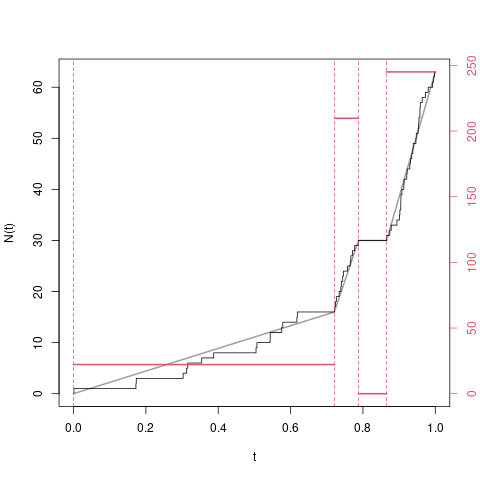
\includegraphics[width=.45\textwidth, trim=0 10 0 50, clip=]{\figcp/FigSegPP-Kilauea-Seg}
    \end{tabular}
  \end{tabular}

  \pause
  \paragraph{Segmentation space.} In continuous time, 
  $$
  \Tcal = \{\tau \in [0, 1]^{K-1}: 0 < \tau_1 < \dots \tau_{K-1} < 1\}
  $$
  so DP does not apply
}

%====================================================================
\frame{\frametitle{Change-point detection in a Poisson process} 

  \bigskip
  \begin{tabular}{cc}
    \hspace{-.04\textwidth}
    \begin{tabular}{p{.5\textwidth}}
      \refer{DLR23}: $\Tcal$ can be partitioned according to the number of events in each segment:
      $$
      \Tcal = \bigcup_\nu \Tcal_\nu,
      $$
      where
      $$
      \Tcal_\nu = \{\tau \in [0, 1]^{K-1}: \forall k, N(\tau_k) - N(\tau_{k-1}) = \nu_k\}
      $$
      
      \pause \bigskip \bigskip 
      \paragraph{Right:} $K = 3$, $\tau = (\tau_1, \tau_2)$, $N(T) = 10$.
      \bigskip ~ 
    \end{tabular}
    & 
    \hspace{-.05\textwidth}
    \begin{tabular}{p{.5\textwidth}}
      \includegraphics[width=.45\textwidth, trim=0 0 20 50, clip=]{\figcp/FigSegPPP-simul-n10-K1-seed1-Contrast}
    \end{tabular}
  \end{tabular}

  \pause 
  \begin{itemize}
    \setlength{\itemsep}{1\baselineskip}
    \item Classical contrasts are {\sl concave} wrt to $\tau$ in each $\Tcal_\nu$;
    \item Optimal change points are located at event times:
    $$
    \widehat{\tau} \in \{T_1, T_2^-, T_2, \dots T_{N(T)}^-\}^{K-1};
    $$
    \item $\widehat{\tau}$ can be recovered by DP in $O(N(T)^2)$.
  \end{itemize}
  
}

%====================================================================
\frame{\frametitle{Change-point detection in a Poisson process: Model selection} 

  \paragraph{Thinning property of Poisson processes.} 
  \begin{tabular}{cc}
    \hspace{-.04\textwidth}
    \begin{tabular}{p{.5\textwidth}}
      \begin{itemize}
        \setlength{\itemsep}{1.1\baselineskip}
        \item $\{N(t)\} \sim PP(\lambda(t))$
        \item \textcolor{blue}{Sample event times} (with prob. $v$) 
        \item \textcolor{red}{Store the remaining events}
      \end{itemize}
    \end{tabular}
    & 
    \hspace{-.1\textwidth}
    \begin{tabular}{p{.4\textwidth}}
      \begin{overprint}
        \onslide<1>
        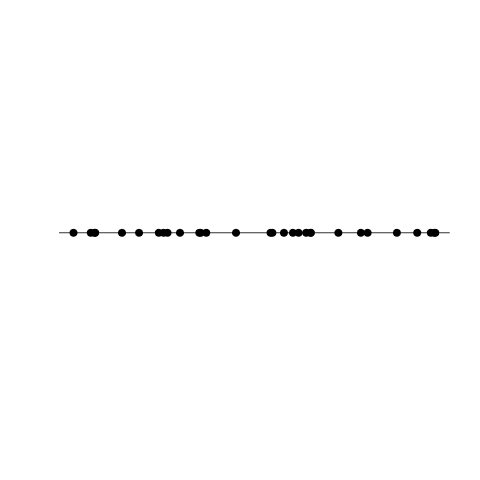
\includegraphics[width=.5\textwidth, trim=50 225 0 225, clip=]{\figcp/FigSegPP-ThiningOriginal.png}
        \onslide<2->
        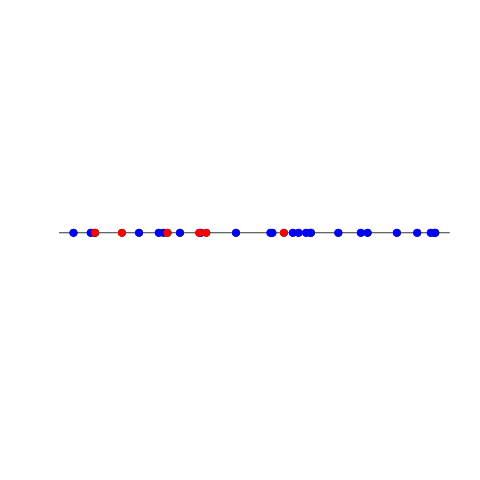
\includegraphics[width=.5\textwidth, trim=50 225 0 225, clip=]{\figcp/FigSegPP-ThiningSampling.png}
      \end{overprint}
    \end{tabular}
  \end{tabular}
  \pause
  $
  ~ \quad 
  \textcolor{blue}{\{N^L(t)\}} \sim PP(v\lambda(t)), \qquad
  \textcolor{red}{\{N^T(t)\}} \sim PP((1-v)\lambda(t)), \qquad
  \textcolor{blue}{\{N^L(t)\}} \perp \textcolor{red}{\{N^T(t)\}}
  $
  
  \bigskip \bigskip \bigskip \pause
  \paragraph{Consequence.} If $\lambda(t)$ piece-wise constant with change-points $\tau = (\tau_k)$ and intensities $\lambda = (\lambda_k)$, then \\ 
  \begin{itemize}
    \setlength{\itemsep}{1\baselineskip}
    \item $\textcolor{blue}{\lambda^L(t)}$ piece-wise constant with change-points $(\textcolor{blue}{\tau_k})$ and intensities $(\textcolor{blue}{v \lambda_k})$, 
    \item $\textcolor{red}{\lambda^T(t)}$ piece-wise constant with change-points $(\textcolor{red}{\tau_k})$ and intensities $(\textcolor{red}{(1-v) \lambda_k})$, 
    \item $\{N^L(t)\}$ and $\{N^T(t)\}$ are independent.
  \end{itemize} 
  
}

%====================================================================
\frame{\frametitle{Change-point detection in a Poisson process: Model selection} 

  \bigskip 
  \begin{tabular}{cc}
    \hspace{-.04\textwidth}
    \begin{tabular}{p{.5\textwidth}}
      \paragraph{Thinning property =} \\
      ~ \\
      ideal setting for cross-validation, because of the independence of $\{N^L(t)\}$ and $\{N^T(t)\}$.

      \bigskip \bigskip 
      \paragraph{Model selection.} \\
      ~ \\
      Choose $K$ using cross-validation \refer{DLR23}.
    \end{tabular}
    & 
    \hspace{-.02\textwidth}
    \begin{tabular}{p{.5\textwidth}}
      \paragraph{Kilauea's eruptions} \\
      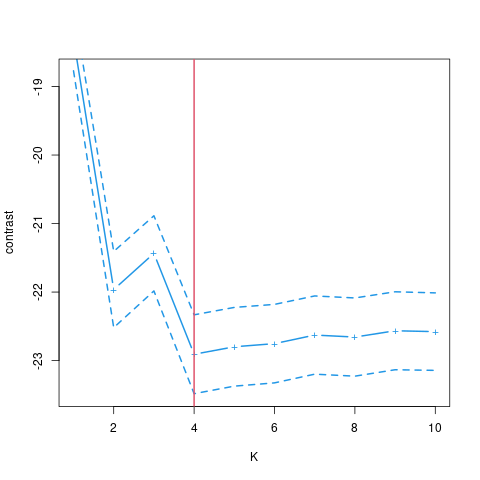
\includegraphics[width=.4\textwidth, trim=0 10 10 10, clip=]{\figcp/FigSegPP-Kilauea-CV-PGtrain}
    \end{tabular}
  \end{tabular}


}

% %====================================================================
% %====================================================================
% \section{Change-point detection in a Poisson process: Extensions}
%====================================================================
\frame{\frametitle{Change-point detection in a Poisson process: Extensions} 

  \bigskip
  \onslide+<1->{\paragraph{Marked Poisson process:} a mark $X_i$ is associated with each event time $T_i$.
  \medskip
  \begin{itemize}
    \item Provided the marks are independent, with segment-dependent distributions, the whole machinery (inference + model selection) applies \refer{DLR23}.
  \end{itemize}}

  \bigskip \bigskip 
  \begin{tabular}{cc}
    \hspace{-.04\textwidth}
    \begin{tabular}{p{.5\textwidth}}
      \onslide+<2->{\paragraph{Segmentation and classification.} \\
      Cluster segments according to different underlying behaviors.}      

      \bigskip 
      \onslide+<3->{\paragraph{Reduced number $L < K$ of intensities:}
      $$
      \lambda_k \in \{\mu_1, \dots, \mu_L\}
      $$
      and $\pi_\ell = \Pr\{\lambda_k = \mu_\ell\}$.}
      
      \bigskip 
      \onslide+<4>{
      \paragraph{Estimation:} EM algorithm including DP for the estimation (M) step \refer{PRL07}.
      ~\bigskip ~\bigskip ~\bigskip ~}
    \end{tabular}
    & 
    \hspace{-.05\textwidth}
    \begin{tabular}{p{.5\textwidth}}
      \begin{overprint}
        \onslide<2>
         \paragraph{Kilauea's eruptions}  \\
        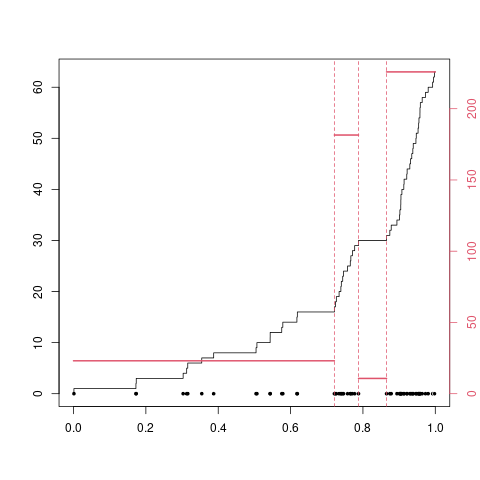
\includegraphics[width=.45\textwidth, trim=0 10 0 50, clip=]{\figcp/FigSeg-HCERES-Kilauea-seg}
        \onslide<3->
         \paragraph{Kilauea's eruptions}  \\
        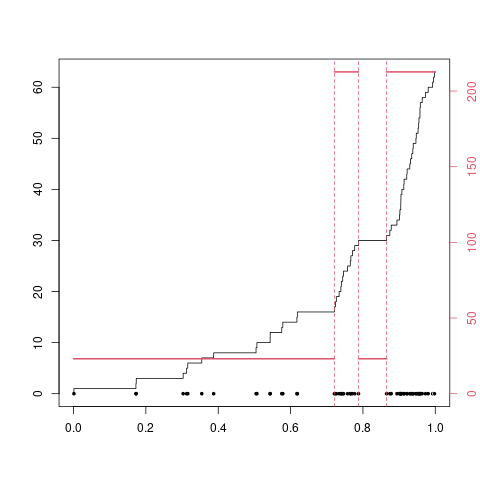
\includegraphics[width=.45\textwidth, trim=0 10 0 50, clip=]{\figcp/FigSeg-HCERES-Kilauea-clustSeg}
      \end{overprint}
    \end{tabular}
  \end{tabular}
  
}

% %====================================================================
% %====================================================================
% \section{Segmentation and classification in a Hawkes process}
%====================================================================
\frame{\frametitle{Segmentation in a Hawkes process} 

  \paragraph{Modeling.} Many counting processes display a self-exciting behavior (events generate --~or prevent~-- new events), which the Poisson process does not account for.
  
  \pause \bigskip \bigskip
  \paragraph{Hawkes process.} Counting process $N(t)$ with intensity conditional on the past events:
  $$
  \lambda(t) 
  = m + \int_0^t h(t-s) d N(s) 
  = m + \sum_{i: T_i < t} h(t -T_i).
  $$
  \begin{itemize}
    \item $m =$ baseline intensity,
    \item $h =$ kernel, e.g. exponential: $h(u) = a e^{-bu}$.
  \end{itemize}

  \pause \bigskip \bigskip 
  \paragraph{Change point detection in the baseline.} Change-points $0 < \tau_1 < \dots < \tau_{K-1} < 1$:
  $$
  \lambda(t) 
  = m_k + \sum_{i: T_i < t} h(t -T_i), 
  \qquad \text{if} \quad
  \tau_{k-1} < t \leq \tau_k.
  $$

}

%====================================================================
\frame{\frametitle{Segmentation in a Hawkes process: Discrete time} 

  \paragraph{Non-additive contrast.} Disjoint time segments are not independent, so  classical contrasts (e.g. negative log-likelihood, \dots) are not additive anymore.

  \pause \bigskip \bigskip 
  \paragraph{Discrete time Hawkes process.} Consider discrete times $t_i = i/n$ and define
  $$
  Y_i \sim \Pcal\left(\mu + \sum_{j \geq 1} \alpha \beta^j Y_{i-j}\right)
  $$
  (taking $\mu = m/n$,  $\beta = e^{-b/n}$).

  \pause \bigskip \bigskip 
  \paragraph{Makovian reformulation.} 
  \begin{itemize}
    \setlength{\itemsep}{1\baselineskip}  
    \item $\{Y_i\}_{i \geq 1}$ is not a Markov chain,
    \item but, defining $U_1 = 0$ and
    $$
    U_i = \beta \left(\alpha Y_{i-1} + U_{i-1}\right),
    \qquad \text{for} \quad i \geq 1,
    $$
    $\{(Y_i, U_i)\}_{i \geq 1}$ is a Markov chain.
  \end{itemize}
  
}

%====================================================================
\frame{\frametitle{Segmentation and classification in a Hawkes process: Discrete time} 

  \paragraph{Hidden Markov models (HMM)} provide a convenient framework for segmentation and classification.
  
  \pause \bigskip \bigskip
  \paragraph{Discrete time Hawkes HMM.}   
  \begin{itemize}
    \setlength{\itemsep}{1\baselineskip}  
    \item Hidden path: $\{Z_i\}_{i \leq 1} =$ homogeneous Markov chain, with transition matrix $\pi$, 
    \item 'Observed path': for $i \geq 1$, set $U_1 = 0$ and
    $$
    Y_i \sim \Pcal\left(\mu_{Z_i} + \sum_{j \geq 1} \alpha \beta^j Y_{i-j}\right), 
    \qquad \qquad 
    U_i = \alpha Y_{i-1} + \beta U_{i-1}.
    $$
  \end{itemize}

  \pause \bigskip
  \paragraph{Inference.} Regular EM algorithm for HMM.


  \pause \bigskip \bigskip
  \paragraph{Extensions.}
  \begin{itemize}
    \item Multivariate (discrete time) Hawkes process.
    \item Applications: neuro-sciences, ecology.
  \end{itemize}

}

%====================================================================
\frame[allowframebreaks]{ \frametitle{References}
  {
   \footnotesize
   \bibliography{/home/robin/Biblio/BibGene}
   \bibliographystyle{alpha}
  }
}

%====================================================================
\backupbegin
%====================================================================

%====================================================================
\frame{\frametitle{HMM for discrete time Hawkes process} 

  \renewcommand{\nodesize}{2em}
  \renewcommand{\edgeunit}{3*\nodesize}

  \paragraph{Graphical model.} 
  
  \begin{center}
  \begin{tikzpicture}
\node[] (Zt_2) at (-\edgeunit, \edgeunit) {}; 
\node[] (Zt_1) at (0, \edgeunit) {$Z_{i-1}$}; 
\node[] (Zt) at (\edgeunit, \edgeunit) {$Z_{i}$}; 
\node[] (Zt1) at (2*\edgeunit, \edgeunit) {$Z_{i+1}$}; 
\node[] (Zt2) at (3*\edgeunit, \edgeunit) {}; 
\node[] (Ut_1) at (-0.5*\edgeunit, 0.5*\edgeunit) {$U_{i-1}$}; 
\node[] (Ut) at (0.5*\edgeunit, 0.5*\edgeunit) {$U_{i}$}; 
\node[] (Ut1) at (1.5*\edgeunit, 0.5*\edgeunit) {$U_{i+1}$}; 
\node[] (Ut2) at (2.5*\edgeunit, 0.5*\edgeunit) {$U_{i+2}$}; 
\node[] (Ut3) at (3.5*\edgeunit, 0.5*\edgeunit) {}; 
\node[] (Yt_2) at (-\edgeunit, 0) {}; 
\node[] (Yt_1) at (0, 0) {$Y_{i-1}$}; 
\node[] (Yt) at (\edgeunit, 0) {$Y_{i}$}; 
\node[] (Yt1) at (2*\edgeunit, 0) {$Y_{i+1}$}; 
\node[] (Yt2) at (3*\edgeunit, 0) {}; 

\draw[->,dashed] (Zt_2) -- (Zt_1); \draw[->] (Zt_1) -- (Zt); \draw[->] (Zt) -- (Zt1); \draw[->,dashed] (Zt1) -- (Zt2);
\draw[->] (Zt_1) -- (Yt_1); \draw[->] (Zt) -- (Yt); \draw[->] (Zt1) -- (Yt1);
\draw[->] (Ut_1) -- (Yt_1); \draw[->] (Ut) -- (Yt); \draw[->] (Ut1) -- (Yt1);
\draw[->] (Ut_1) -- (Ut); \draw[->] (Ut) -- (Ut1); \draw[->] (Ut1) -- (Ut2); \draw[->,dashed] (Ut2) -- (Ut3);
\draw[->,dashed] (Yt_2) -- (Ut_1); \draw[->] (Yt_1) -- (Ut); \draw[->] (Yt) -- (Ut1); \draw[->] (Yt1) -- (Ut2);
\end{tikzpicture}


  \end{center}
}

%====================================================================
\backupend
%====================================================================

%====================================================================
%====================================================================
\end{document}
%====================================================================
%====================================================================
  
  \begin{tabular}{cc}
    \hspace{-.04\textwidth}
    \begin{tabular}{p{.5\textwidth}}
    \end{tabular}
    & 
    \hspace{-.02\textwidth}
    \begin{tabular}{p{.5\textwidth}}
    \end{tabular}
  \end{tabular}

